\documentclass[10pt,a4paper,final]{article}
% cestina a fonty

\usepackage[utf8]{inputenc}
\usepackage[T1]{fontenc}
\usepackage{lmodern}
\usepackage{textcomp}
\usepackage{times}
% odsazeni prvniho radku
\usepackage{indentfirst}
% balicky pro odkazy
\usepackage[bookmarksopen,colorlinks,plainpages=false,urlcolor=blue,
unicode,linkcolor=black]{hyperref}
\usepackage{url}
% obrazky
\usepackage[dvipdf]{graphicx}
% velikost stranky
\usepackage[top=3.0cm, left=2.5cm, text={17cm, 24cm}, ignorefoot]{geometry}
\usepackage{graphicx}
	\usepackage{graphics}
	\usepackage{picture}
	\usepackage{epstopdf}

\begin{document}

%%%%%%%%%%%%%%%%%%%%%%%%%%%%%%%%%%%%%%%%%%%%%%%%%%%%%%%%%%%%%%%%%%%%%%%%%%%%%%%%

  % nastaveni cislovani
  \pagestyle{plain}
  \pagenumbering{arabic}
  \setcounter{page}{1}
  
  % nastaveni mezery mezi odstavci a odsazeni prvniho radku
  \setlength{\parindent}{1cm}
  \setlength{\parskip}{0.2cm plus4mm minus3mm}
  
  \noindent
  Dokumentácia Projektu 2: Prenos súborov v C/C++ do IPK 2015/2016 \\
  Meno a priezvisko: Peter Tisovčík \\
  Login: xtisov00 \\
  


%%%%%%%%%%%%%%%%%%%%%%%%%%%%%%%%%%%%%%%%%%%%%%%%%%%%%%%%%%%%%%%%%%%%%%%%%%%%%%%%
  \section{Úvod} \label{uvod}
%%%%%%%%%%%%%%%%%%%%%%%%%%%%%%%%%%%%%%%%%%%%%%%%%%%%%%%%%%%%%%%%%%%%%%%%%%%%%%%%

Táto dokumentácia popisuje implementáciu servera a klienta v jazyku C/C++. Zadaný projekt slúži pre vytvorenie konkurentného serveru a klienta, ktorý bude s ním komunikovať pomocou schránok(sockets API) a vytvoreného aplikačného protokolu. Server a klient si možu medzi sebou vymieňať súbory(upload, download). 

%%%%%%%%%%%%%%%%%%%%%%%%%%%%%%%%%%%%%%%%%%%%%%%%%%%%%%%%%%%%%%%%%%%%%%%%%%%%%%%%
  \section{Implementácia} \label{implementacia}
%%%%%%%%%%%%%%%%%%%%%%%%%%%%%%%%%%%%%%%%%%%%%%%%%%%%%%%%%%%%%%%%%%%%%%%%%%%%%%%%

Po spustení serveru začne server čakať na klientov a vybabovať ich požiadavky na základe správ, ktoré obdrží. 

V prípade, že chce klient stiahnuť súbor so serveru,
musí odoslať správu s požadovanou požiadavkou a názvom súboru,
ktorý chce klient stiahnuť. Server príjme správu načíta a uloží
si súbor do pamäte, uzavrie súbor a pošle odpoveď s veľkosťou
súboru, aby klient vedel, koľko údajov má prijať. Následne mu klient
odpovie, že dostal požadované údaje o veľkosti a server začne posielať údaje.
V prípade, že server neobsahuje daný súbor alebo nemá dostatočné
oprávnenia na jeho čítanie, tak pošle server klientovi namiesto veľkosti
súboru správu o chybe a klient vypíše túto chybu a ukončí sa.

Server a klient kontroluje zadanie nesprávnych argumentov, ich duplicitu,
nevalidný port, chyby pri pripojení na daný host alebo na daný port,
chyby pri posielaní údajov, otváraní súborov. Podporujú spustenie
v rovnakom adresári a poslanie alebo nahranie súboru v danom adresári
ale len pre jedného klienta, pre viacerých klientov, ktorý žiadajú
o rovnaký súbor nie je zaručené, že bude požiadavka úspešná. Klient
a server nepodporujú ukončenie spojenia počas komunikácie, procesy
zostanú čakať na danú správu/dáta.

Spoločné funkcie sa nachádzajú v súbore \texttt{common.cpp} a \texttt{common.h}. Medzi spoločné funkcie patrí zistenie typu správy, výpis chyby, prečítanie správy, vytvorenie spravy, zistenie veľkosti spravý a chybové kódy.
\\\\
\texttt{server -p port}\\
\texttt{client -p port -h hostname [{-u|-d}] {file\_name}}\\\\
\texttt{server -p 8008}\\
\texttt{client -p 8008 -h localhost {-u} {file\_name}}\\
\texttt{client -p 8008 -h localhost {-d} {file\_name}}\\



\begin{figure}[ht]
\begin{center}
\scalebox{0.34}
{	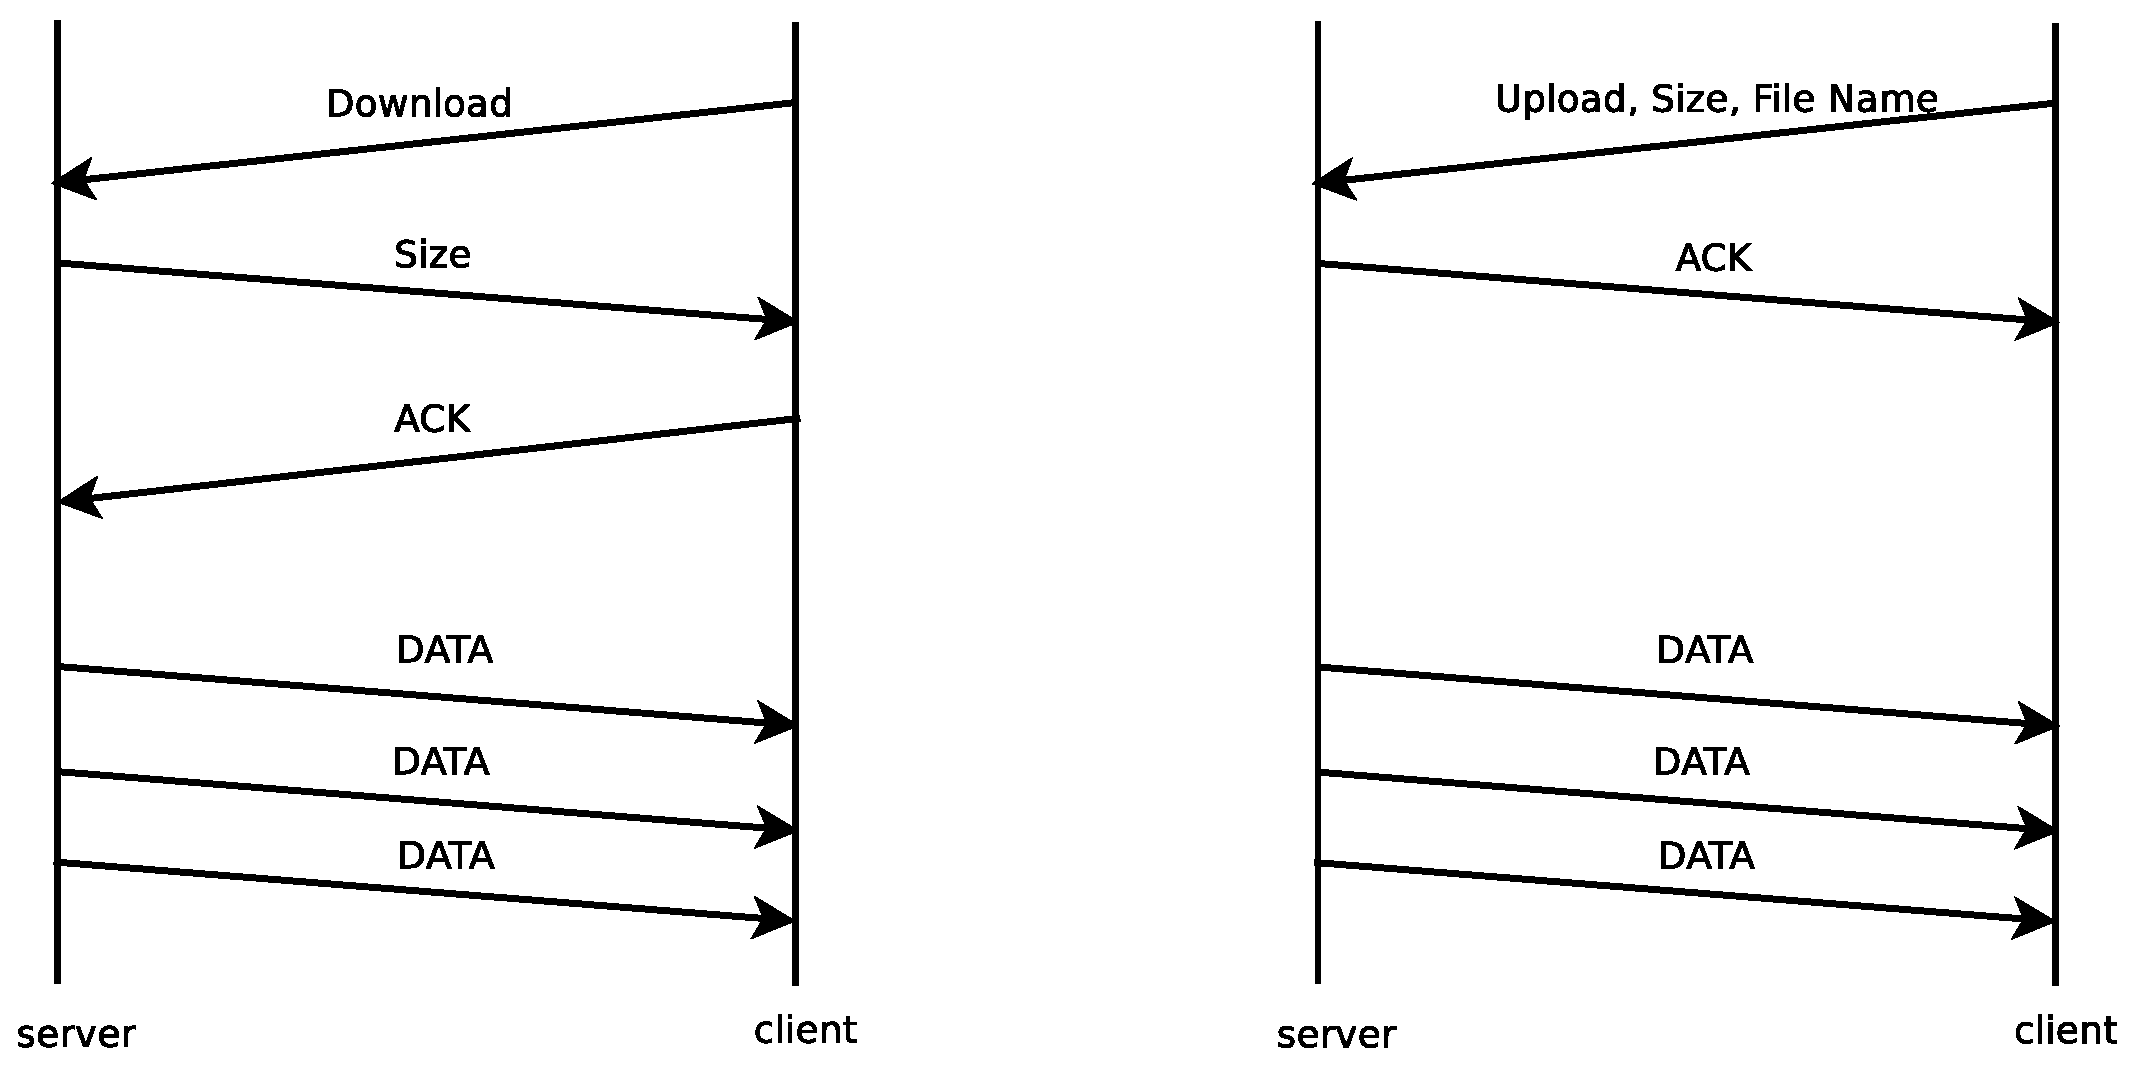
\includegraphics{Diagram1.eps}
	}
\caption{Popis zasielania správ pri komunikácií}
\label{etiopan}
\end{center}
\end{figure}


    
\end{document}
